\documentclass[tikz,border=8pt]{standalone}
\usepackage{amsmath,amssymb}
\usetikzlibrary{arrows.meta,calc,decorations.pathreplacing,patterns,shapes.geometric,positioning,shadings}

\begin{document}
\begin{tikzpicture}[
  >=Stealth,
  thick,
  font=\footnotesize
]

% ============================================================
% LEFT PANEL: Ray splitting at interface
% ============================================================
\begin{scope}[shift={(0,0)}]

  % Upper medium (air)
  \fill[blue!4] (-4.2,0) rectangle (2.2,3.2);
  % Lower medium (glass)
  \fill[red!6] (-4.2,-3.2) rectangle (2.2,0);

  % Interface line
  \draw[black, line width=0.8pt] (-4.2,0) -- (2.2,0);

  % Medium labels
  \node[anchor=west, font=\small] at (-4.15,2.85) {Air \ $n_1=1$};
  \node[anchor=west, font=\small] at (-4.15,-2.9) {Glass \ $n_2=1.5$};

  % Normal (dashed, vertical)
  \draw[gray!70, dashed, line width=0.6pt] (0,-2.7) -- (0,2.7);
  \node[gray!70, anchor=south, font=\scriptsize] at (0,2.72) {normal};

  % Angles (theta_i = 60 deg, theta_t = arcsin(sin60/1.5) = 35.26 deg)
  % Incident ray: from upper-left, angle 60 deg from normal
  % Direction vector for incident (coming toward origin): going from (-sin60*L, cos60*L) to origin
  % L = 2.6
  \pgfmathsetmacro{\thi}{60}
  \pgfmathsetmacro{\tht}{35.264389}
  \pgfmathsetmacro{\Ri}{2.6}
  \pgfmathsetmacro{\Rr}{2.4}
  \pgfmathsetmacro{\Rt}{2.5}

  % Incident ray (black, thick) from upper-left toward origin
  \coordinate (I) at ({-\Ri*sin(\thi)}, {\Ri*cos(\thi)});
  \draw[black, line width=1.2pt, -{Stealth[length=2.6mm]}] (I) -- (-0.02,0);

  % Reflected ray (blue) toward upper-right
  \coordinate (R) at ({\Rr*sin(\thi)}, {\Rr*cos(\thi)});
  \draw[blue!70!black, line width=1.2pt, -{Stealth[length=2.6mm]}] (0,0) -- (R);

  % Refracted ray (red) toward lower-right
  \coordinate (T) at ({\Rt*sin(\tht)}, {-\Rt*cos(\tht)});
  \draw[red!75!black, line width=1.2pt, -{Stealth[length=2.6mm]}] (0,0) -- (T);

  % Angle arcs
  \draw[black, line width=0.5pt] (0,0.9) arc[start angle=90, end angle=150, radius=0.9];
  \node[font=\scriptsize] at ({-0.55*sin(60)-0.08}, {0.55*cos(60)+0.55}) {$\theta_i$};

  \draw[blue!70!black, line width=0.5pt] (0,0.9) arc[start angle=90, end angle=30, radius=0.9];
  \node[blue!70!black, font=\scriptsize] at ({0.55*sin(60)+0.1}, {0.55*cos(60)+0.55}) {$\theta_r$};

  \draw[red!75!black, line width=0.5pt] (0,-0.95) arc[start angle=-90, end angle=-90+35.264, radius=0.95];
  \node[red!75!black, font=\scriptsize] at ({0.7*sin(35.264)+0.12}, {-0.7*cos(35.264)-0.02}) {$\theta_t$};

  % Polarization indicators on incident ray midpoint
  \coordinate (IM) at ({-0.55*\Ri*sin(\thi)}, {0.55*\Ri*cos(\thi)});
  % s-polarization: dot into page (circle with dot)
  \draw[black, line width=0.5pt, fill=white] (IM) circle (2.0pt);
  \fill[black] (IM) circle (0.5pt);
  \node[anchor=east, font=\scriptsize] at ([xshift=-0.12cm]IM) {$s$};

  % p-polarization: double-arrow in incidence plane, perpendicular to ray
  % Ray direction (from I toward origin): (sin60, -cos60). Perpendicular in plane: (cos60, sin60)
  \coordinate (IP) at ({-0.35*\Ri*sin(\thi)}, {0.35*\Ri*cos(\thi)});
  \pgfmathsetmacro{\px}{0.32*cos(\thi)}
  \pgfmathsetmacro{\py}{0.32*sin(\thi)}
  \draw[black, line width=0.7pt, {Stealth[length=1.8mm]}-{Stealth[length=1.8mm]}]
    ({-0.35*\Ri*sin(\thi)-\px}, {0.35*\Ri*cos(\thi)-\py}) --
    ({-0.35*\Ri*sin(\thi)+\px}, {0.35*\Ri*cos(\thi)+\py});
  \node[anchor=west, font=\scriptsize] at ({-0.35*\Ri*sin(\thi)+\px+0.04}, {0.35*\Ri*cos(\thi)+\py+0.02}) {$p$};

  % Ray labels
  \node[anchor=south east, font=\scriptsize] at ([xshift=-2pt,yshift=2pt]I) {incident};
  \node[anchor=south west, blue!70!black, font=\scriptsize] at ([xshift=2pt,yshift=2pt]R) {reflected};
  \node[anchor=north west, red!75!black, font=\scriptsize] at ([xshift=2pt,yshift=-2pt]T) {refracted};

  % Side annotations (formulas)
  \node[anchor=north west, font=\scriptsize, align=left] at (-4.2,-3.35)
    {$n_1 \sin\theta_i = n_2 \sin\theta_t$};
  \node[anchor=north west, font=\scriptsize, align=left] at (-4.2,-3.85)
    {$R_\perp = \left(\dfrac{n_1-n_2}{n_1+n_2}\right)^{\!2}\!=0.04$ \ (normal)};
  \node[anchor=north west, font=\scriptsize, align=left] at (-4.2,-4.65)
    {TIR: $\sin\theta_c = n_2/n_1$ \ (dense $\to$ rare)};

  % Panel title
  \node[font=\small\bfseries, anchor=south] at (-1,3.35) {(a) Ray splitting};

\end{scope}

% ============================================================
% RIGHT PANEL: Reflectance curves R_s, R_p vs theta_i
% ============================================================
\begin{scope}[shift={(7.5,-0.2)}]

  % Plot area: x 0..90 deg mapped to 0..6.4 cm; y 0..1 mapped to 0..5.4 cm
  \pgfmathsetmacro{\XS}{6.4/90}
  \pgfmathsetmacro{\YS}{5.4/1}

  % Axes
  \draw[->, line width=0.7pt] (0,-2.5) -- (7.0,-2.5) node[anchor=west, font=\scriptsize] {$\theta_i$};
  \draw[->, line width=0.7pt] (0,-2.5) -- (0, 3.2) node[anchor=south, font=\scriptsize] {$R$};

  % x ticks
  \foreach \t in {0,30,60,90} {
    \pgfmathsetmacro{\xt}{\t*\XS}
    \draw[line width=0.5pt] (\xt,-2.5) -- (\xt,-2.6);
    \node[anchor=north, font=\scriptsize] at (\xt,-2.62) {$\t^\circ$};
  }
  % y ticks
  \foreach \y/\yl in {0/0, 0.25/0.25, 0.5/0.5, 0.75/0.75, 1/1} {
    \pgfmathsetmacro{\yt}{-2.5+\y*\YS}
    \draw[line width=0.5pt] (0,\yt) -- (-0.08,\yt);
    \node[anchor=east, font=\scriptsize] at (-0.1,\yt) {$\yl$};
  }

  % R_s curve (blue, monotonically increasing)
  % Sampled points computed with n1=1, n2=1.5
  \draw[blue!70!black, line width=1.2pt]
    plot coordinates {
      ( 0.000, {-2.5+ 0.0400*\YS})
      ( 5.000, {-2.5+ 0.0402*\YS})
      (10.000, {-2.5+ 0.0412*\YS})
      (15.000, {-2.5+ 0.0428*\YS})
      (20.000, {-2.5+ 0.0454*\YS})
      (25.000, {-2.5+ 0.0491*\YS})
      (30.000, {-2.5+ 0.0542*\YS})
      (35.000, {-2.5+ 0.0611*\YS})
      (40.000, {-2.5+ 0.0704*\YS})
      (45.000, {-2.5+ 0.0830*\YS})
      (50.000, {-2.5+ 0.1000*\YS})
      (55.000, {-2.5+ 0.1234*\YS})
      (60.000, {-2.5+ 0.1562*\YS})
      (65.000, {-2.5+ 0.2034*\YS})
      (70.000, {-2.5+ 0.2738*\YS})
      (75.000, {-2.5+ 0.3832*\YS})
      (80.000, {-2.5+ 0.5595*\YS})
      (85.000, {-2.5+ 0.7560*\YS})
      (89.000, {-2.5+ 0.9470*\YS})
      (90.000, {-2.5+ 1.0000*\YS})
    };

  % R_p curve (red, dips to zero at theta_B ~= 56.31, then rises)
  \draw[red!80!black, line width=1.2pt]
    plot coordinates {
      ( 0.000, {-2.5+ 0.0400*\YS})
      ( 5.000, {-2.5+ 0.0394*\YS})
      (10.000, {-2.5+ 0.0376*\YS})
      (15.000, {-2.5+ 0.0347*\YS})
      (20.000, {-2.5+ 0.0305*\YS})
      (25.000, {-2.5+ 0.0253*\YS})
      (30.000, {-2.5+ 0.0193*\YS})
      (35.000, {-2.5+ 0.0128*\YS})
      (40.000, {-2.5+ 0.0067*\YS})
      (45.000, {-2.5+ 0.0020*\YS})
      (50.000, {-2.5+ 0.0001*\YS})
      (53.000, {-2.5+ 0.0010*\YS})
      (56.310, {-2.5+ 0.0000*\YS})
      (58.000, {-2.5+ 0.0024*\YS})
      (60.000, {-2.5+ 0.0074*\YS})
      (65.000, {-2.5+ 0.0342*\YS})
      (70.000, {-2.5+ 0.0925*\YS})
      (75.000, {-2.5+ 0.2024*\YS})
      (80.000, {-2.5+ 0.3883*\YS})
      (85.000, {-2.5+ 0.6614*\YS})
      (89.000, {-2.5+ 0.9348*\YS})
      (90.000, {-2.5+ 1.0000*\YS})
    };

  % Brewster angle marker: dashed vertical from zero point to x-axis
  \pgfmathsetmacro{\xB}{56.31*\XS}
  \draw[gray, dashed, line width=0.5pt] (\xB,-2.5) -- (\xB,{-2.5+0.9*\YS});
  \fill[red!80!black] (\xB,-2.5) circle (1.5pt);
  \node[anchor=north, font=\scriptsize, red!80!black] at (\xB,-2.62) {};
  \node[anchor=south, font=\scriptsize, red!80!black] at (\xB,{-2.5+0.9*\YS}) {};
  % Brewster label on axis
  \node[anchor=north, font=\scriptsize, red!80!black] at (\xB,-2.95) {$\theta_B\!=\!56.3^\circ$};

  % Curve labels
  \node[blue!70!black, anchor=west, font=\scriptsize] at ({82*\XS+0.1},{-2.5+0.58*\YS}) {$R_s$};
  \node[red!80!black, anchor=west, font=\scriptsize] at ({82*\XS+0.1},{-2.5+0.42*\YS}) {$R_p$};

  % Normal-incidence 4% marker
  \draw[gray, dotted, line width=0.4pt] (0,{-2.5+0.04*\YS}) -- ({15*\XS},{-2.5+0.04*\YS});
  \node[anchor=west, font=\scriptsize, gray!60!black] at ({14*\XS},{-2.5+0.12*\YS}) {$4\%$};

  % Side annotation
  \node[anchor=north west, font=\scriptsize, align=left] at (-0.6,-3.35)
    {$\tan\theta_B = n_2/n_1$, \ $R_p(\theta_B)=0$};
  \node[anchor=north west, font=\scriptsize, align=left] at (-0.6,-3.85)
    {$R_s, R_p$ for $n_1\!=\!1 \to n_2\!=\!1.5$};

  % Panel title
  \node[font=\small\bfseries, anchor=south] at (3.2,3.35) {(b) Reflectance $R_s(\theta)$, $R_p(\theta)$};

\end{scope}

\end{tikzpicture}
\end{document}
